\documentclass[11pt,article]{memoir}
\usepackage{multirow}
\usepackage{agd-assignment}
\usepackage{fancybox}
\usepackage{afterpage}
\usepackage{graphicx}
\usepackage{standalone}
\usepackage[yyyymmdd,hhmmss]{datetime}
\usepackage{pdfpages}

\usepackage{listings}
\lstset{
    frame=single,
    breaklines=true,
    postbreak=\raisebox{0ex}[0ex][0ex]{\ensuremath{\color{red}\hookrightarrow\space}}
}
\let\footruleskip\undefined
\usepackage{fancyhdr}
\fancyhf{}
\lhead{\textbf{FRCRCE}}
\rhead{\textbf{DEPARTMENT OF INFORMATION TECHNOLOGY}}

\rfoot{Compiled on \today\ at \currenttime \quad \textbf{\thepage}}
%\pagestyle{fancy}
\assigncourse{Course title: Big Data Analytics}
\assignterm{Course term: 2019-2020}
\assigncat{Practical}
%\assigntitle{}
%\renewcommand{\headrulewidth}{0pt}
%\renewcommand{\footrulewidth}{0pt}}
\lfoot{\textbf{Course title: Big Data Analytics}}

\fancypagestyle{plain}{}
\pagestyle{fancy}
\begin{document}
\sloppy
\fancypage{\doublebox}{}
\begin{flushleft}


    \begin{tabular}{ | p{4cm} | p{5cm} | p{3.5cm} | p{2cm} |}
    \hline

    \textbf{Name of the student:}& Tanmay Prashant Rane &\textbf{Roll No.} & 8031 \\ \hline
    \textbf{Practical Number:}& 10 & \textbf{Date of Practical:} & \\ \hline
	\textbf{Relevant CO's} & \multicolumn{3}{|p{10.5cm}|}{\begin{flushleft}
	\textbf{At the end of the course students will be able to apply big data analytics in real life applications.}
	\end{flushleft}}\\
    \hline
    \multicolumn{3}{|p{12.5cm}|}{\textbf{Sign here to indicate that you have read all the relevant material provided before attempting this practical}}& \textbf{Sign:}\\ \hline
    \end{tabular}
    \vspace{1cm}
        \textbf{Practical grading using Rubrics}
           \textbf{Practical grading using Rubrics}
                             \begin{tabular}{|p{2cm}|p{2cm}|p{2cm}|p{2cm}|p{2cm}|p{2cm}|}
                             \hline \textbf{Indicator} & \textbf{Very Poor} & \textbf{Poor} & \textbf{Average} & \textbf{Good} & \textbf{Excellent} \\ 
                             \hline \textbf{Timeline} (2) & More than a session late (0) & NA  & NA & NA  & Early or on time (2) \\ 
                             \hline \textbf{Code design} (2) & N/A & Very poor code design with no comments and indentation(0.5) & Poor code design with very comments and indentation
                             (1) & Design with good coding standards (1.5) & Accurate design with better coding satndards (2) \\ 
                             \hline \textbf{Performance} (4) & Unable to
                             perform the
                             experiment
                             (0) & Able to
                             partially
                             perform the
                             experiment
                             (1)
                              & Able to
                              perform the
                              experiment
                              for certain use
                              cases (2) & Able to
                              perform the
                              experiment
                              considering
                              most of the
                              use cases (3)
                              & Able to
                              perform the
                              experiment
                              considering
                              all use cases
                              (4) \\ 
                             \hline \textbf{Postlab} (2) & Both answers incorrect (0) & N/A & One answer correct  (1) & N/A & Both answers correct (2) \\ 
                             \hline 
                             \end{tabular}
        %\vspace{-8cm}
        \begin{table}[h!]
        \centering
        \begin{tabular}{|c|c|}
                \hline \textbf{Total Marks (10)} & \textbf{Sign of instructor with date} \\ 
                \hline  &  \\ & \\
                \hline 
                \end{tabular} 
        \end{table}
        
    \pagebreak

	%\input{assignment}

\maketitle

%\thispagestyle{empty}
\hrule \vspace{0.2cm}
\textbf{Problem Statement: To find common friends in social network graph using map-reduce. }\hrule\vspace{0.2cm}
\textbf{Theory:}\hrule\vspace{0.2cm}
\parskip 2mm
Given a social network with tens of millions of users, in this chapter we’ll implement
a MapReduce program to identify “common friends” among all pairs of users. Let U
be a set of all users: {U 1 , U 2 , ..., U n }. Our goal is to find common friends for every pair
of (U i , U j ) where i not equal to j.

These days most social network sites (such as Facebook, hi5, and LinkedIn) offer
services to help you share messages, pictures, and videos among friends. Some sites
even offer video chat services to help you connect with friends. By definition, a friend
is a person whom one knows, likes, and trusts. For example, Facebook has your list of
friends, and friend relationships are bidirectional on the site; if I’m your friend, you’re
mine too. Typically social networks precompute calculations when they can to reduce
the processing time of requests, and one common processing request involves the
“You and Mary (your friend) have 185 friends in common” feature. When you visit
someone’s profile, you see a list of friends that you have in common. This list doesn’t
change frequently, so it is wasteful for the site to recalculate it every time you visit
that person’s profile.

Input

We prepare input as a set of records, where each record has the following format:

<person><,><friend 1 ><friend 2 >...<friend N >

where <friend 1 ><friend 2 > ... <friend N > are friends of the <person> . 

Note that in real projects/applications, each person/friend will be identified as a unique user ID. A very simple and complete example of input is as follows:

100, 200 300 400 500 600\\
200, 100 300 400\\
300, 100 200 400 500\\
400, 100 200 300\\
500, 100 300\\
600, 100\\
In this example, user 500 has two friends identified by the user IDs 100 and 300, and user 600 has only one friend: user 100.

The mapper accepts a (key 1 , value 1 ) pair, where key 1 is a person and value 1 is a list of associated friends of that person. The mapper
emits a set of new (key 2 , value 2 ) pairs; key 2 is a Tuple2(key 1 , friend i ) , where friend i belongs value 1 , and value 2 is the same as value 1 (a list of all friends for key 1 ). The reducer’s key is a pair of two users (User j , User k ) and value is a list of sets of friends. The reduce() function will intersect all sets of friends to find common and mutual friends for the (User j , User k ) pair.
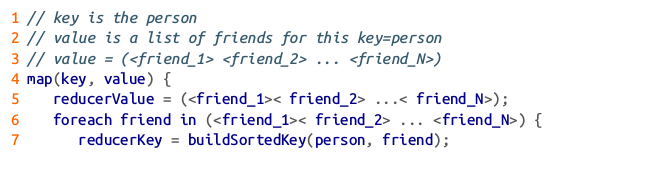
\includegraphics{1.png}
\includepdf[pages={2,3,4,5}]{Theory.pdf}
\afterpage{\newpage}\newpage
\textbf{Code:}\hrule
\vspace{0.5cm}
Write map-reduce code to implement algorithm\\
\textbf{\underline{code for mapper:}}

% Write code of mapper here
\begin{lstlisting}[language=java]
import java.io.IOException;
import java.util.Arrays;
import java.util.HashMap;
import java.util.List;

import org.apache.hadoop.conf.Configuration;
import org.apache.hadoop.fs.Path;
import org.apache.hadoop.io.LongWritable;
import org.apache.hadoop.io.Text;
import org.apache.hadoop.mapreduce.Job;
import org.apache.hadoop.mapreduce.Mapper;
import org.apache.hadoop.mapreduce.Reducer;
import org.apache.hadoop.mapreduce.lib.input.FileInputFormat;
import org.apache.hadoop.mapreduce.lib.output.FileOutputFormat;
import org.apache.hadoop.util.GenericOptionsParser;

public class Map extends Mapper<LongWritable, Text, Text, Text> {

private Text word = new Text();

public void map(LongWritable key, Text value, Context context) throws IOException, InterruptedException {
String[] line = value.toString().split(", ");
if (line.length == 2) {
String friend1 = line[0];
List<String> values = Arrays.asList(line[1].split(" "));
for (String friend2 : values) {
int f1 = Integer.parseInt(friend1);
int f2 = Integer.parseInt(friend2);
if (f1 < f2)
word.set(friend1 + "," + friend2);
else
word.set(friend2 + "," + friend1);
context.write(word, new Text(line[1]));
}
}
}

}
	
\end{lstlisting}
\newpage
\textbf{\underline{Code for Reducer:}}
\begin{lstlisting}[language=java]
public class Reduce extends Reducer<Text, Text, Text, Text> {
private Text result = new Text();

public void reduce(Text key, Iterable<Text> values, Context context) throws IOException, InterruptedException {
HashMap<String, Integer> map = new HashMap<String, Integer>();
StringBuilder sb = new StringBuilder();
for (Text friends : values) {
List<String> temp = Arrays.asList(friends.toString().split(" "));
for (String friend : temp) {
if (map.containsKey(friend))
sb.append(friend + ',');
else
map.put(friend, 1);

}
}
if (sb.lastIndexOf(",") > -1) {
sb.deleteCharAt(sb.lastIndexOf(","));
}

result.set(new Text(sb.toString()));
context.write(key, result);
}
}




\end{lstlisting}

\textbf{\underline{Code for Driver Class:}}
\begin{lstlisting}[language=java]
public class MutualFriends {

public static void main(String[] args) throws Exception {
Configuration conf = new Configuration();
String[] otherArgs = new GenericOptionsParser(conf, args).getRemainingArgs();
// get all args
//		if (otherArgs.length != 2) {
//			System.err.println("Usage: Mutual Friend <inputfile hdfs path> <output file hdfs path>");
//			System.exit(2);
//		}

@SuppressWarnings("deprecation")
Job job = new Job(conf, "MutualFriend");
job.setJarByClass(MutualFriends.class);
job.setMapperClass(Map.class);
job.setReducerClass(Reduce.class);

job.setOutputKeyClass(Text.class);

job.setOutputValueClass(Text.class);
// set the HDFS path of the input data
FileInputFormat.addInputPath(job, new Path("/media/tanmay/Data/SEM-8/BDA/EXP10/bdaexp10/BDAexp10data"));
// set the HDFS path for the output
FileOutputFormat.setOutputPath(job, new Path("/media/tanmay/Data/SEM-8/BDA/EXP10/bdaexp10/out"));
// Wait till job completion
System.exit(job.waitForCompletion(true) ? 0 : 1);
}	

}

\end{lstlisting}

\textbf{Output:}
\newcommand{\tab}[1]{\hspace{.1\textwidth}\rlap{#1}}

100,200		\tab{300,400}\\
100,300		\tab{200,400,500}\\
100,400		\tab{200,300}\\
100,500		\tab{300}\\
100,600		\\
200,300		\tab{100,400}\\
200,400		\tab{100,300}\\
300,400		\tab{100,200}\\
300,500		\tab{100}\\

\newpage
\textbf{PostLab:}\hrule
Explain applications of above code in Facebook as social network\\
\textbf{\underline{Answer for postlab question}}                        

Facebook is the latest in a long line of what we now know as “social networking” websites. But what sets it apart from the competitors, is its popularity. At last check, Facebook boasts over 2.23 billion active users.

With a billion users and requirements to analyze more than 105 terabytes every 30 minutes, Facebook's appetite for crunching data has reached very huge proportions.

Hadoop is the key tool Facebook uses, not simply for analysis, but as an engine to power many features of the Facebook site, including messaging. That multitude of monster workloads drove the company to launch its Prism project, which supports geographically distributed Hadoop data stores.

\noindent Applications of above code for Facebook are as follows:

\begin{enumerate}
	\item Finding mutual friends of two users instantly
	\item Establishing suggestions for friendship on basis of mutual friends
	\item Suggesting adds that mutual friends see to the group of friends
	\item Constructing the "you may know section"
	\item Pushing activities to feed that happened in cluster of particular group
	\item Suggesting games and online challenges
\end{enumerate}
                        
\newpage
Explain applications of above code in LinkedIn as social network\\
\textbf{\underline{Answer for postlab question}}

With more than 400 million profiles (122 million in US and 33 million in India) across 200+ countries, more than 100 million unique monthly visitors, 3 million company pages, 2 new members joining the network every second, 5.7 billion professional searches in 2012,7600 full-time employees, \$780 million revenue as of Oct, 2015 and earnings of 78 cents per share LinkedIn is the largest social network for professionals. People prefer to share their expertise and connect with like-minded professionals to discuss various issues of interest in a platform like LinkedIn, as it allows them to represent themselves formally in a less traditional manner. 2 or more people join LinkedIn’s professional network every second, making up the pool of 400 million members

\begin{enumerate}
	\item People you may know
	\item Jobs you maybe interested in
	\item News Feed Updates
	\item Skill Endorsements
	\item Pushing activities to feed that happened in cluster of particular group
	\item Suggesting games and online challenges
\end{enumerate}
    

\end{flushleft}
\end{document}

